\documentclass{article}
\usepackage[utf8]{inputenc}
\usepackage{minted}
\usepackage{graphicx}
\usepackage{hyperref}
\usepackage[dvipsnames]{xcolor}
\usepackage{comment}

\title{pycom lopy4 loramac prise en main}
\author{cmonaton }
\date{July 2019}

\begin{document}











\maketitle


\section{Introduction}
But : se connecter à la carte pour télécharger un firmware puis faire communiquer 2 cartes directement en LoRa MAC c.à.d sans passer par le réseau LoRaWAN.\\
Carte : pycom lopy 4 avec expansion board V3.0

\begin{figure}[H]
  \centering
  \begin{minipage}[b]{0.4\textwidth}
    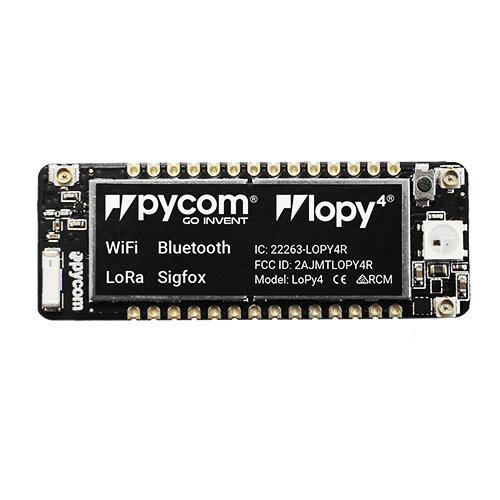
\includegraphics[keepaspectratio=true,scale=1.7]{pycom_lopy4.jpeg}
        \caption{pycom lopy 4}
  \end{minipage}
  \hfill
  \begin{minipage}[b]{0.4\textwidth}
   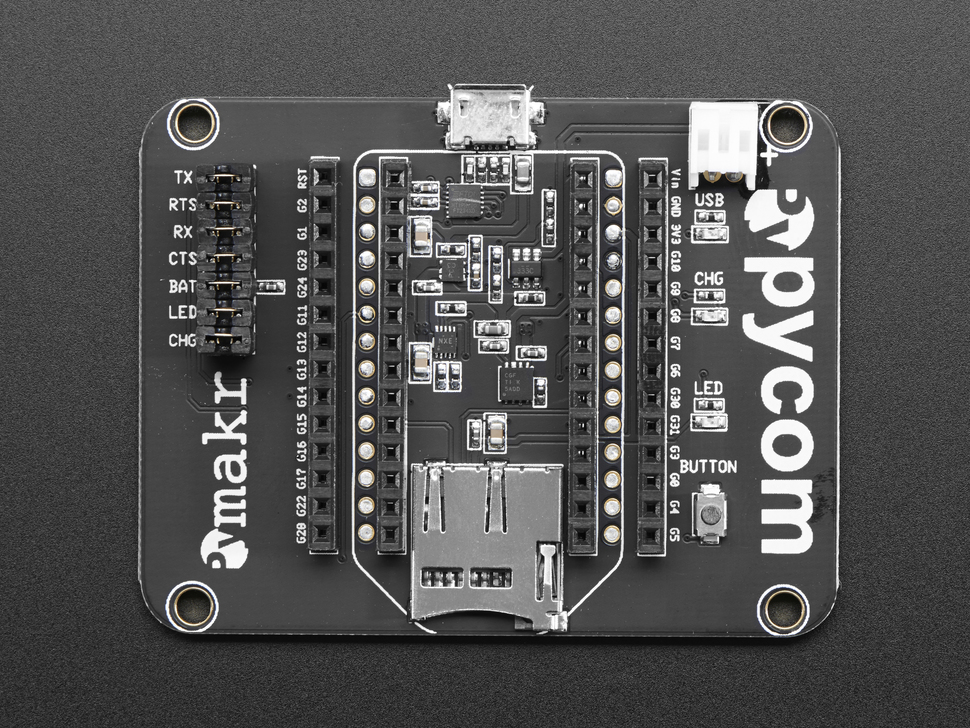
\includegraphics[keepaspectratio=true,scale=0.5]{pycom_expansion_board.jpeg}
    \caption{expansion board v3.0}
  \end{minipage}
\end{figure}

    \begin{figure}[H]
\begin{center}
\advance\leftskip-3cm
\advance\rightskip-3cm
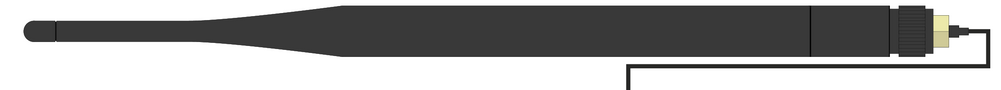
\includegraphics[keepaspectratio=true,scale=0.2]{lora_antenna.png}
\caption{antenne LoRa}
\label{visina8}
\end{center}\end{figure}


\section{Matériel}
\textcolor{red}{Branchez l'antenne LoRa avant d'alimenter la carte sinon la carte grille}


\section{Se connecter à la carte pour la programmer}


\begin{comment}
\subsection{Utiliser Telnet pour se connecter à la carte}

Suivre également sur ce lien : \url{https://docs.pycom.io/gettingstarted/programming/repl/telnet/}

Double cliquer sur l'icône wifi du pycom lopy pour s'y connecter, dans mon cas lopy-wlan-892c

Ouvrir un terminal et taper : telnet 192.168.4.1 \\
login : micro \\
mdp : python \\

\end{comment}


\begin{comment}
\subsubsection{Programmer la carte depuis cette interface}


\begin{enumerate}
    \item Afficher "Hello" : 
    \begin{minted}{python}
variable = "Hello World"
print(variable) 
    \end{minted}

    \item Allumer la led en vert : 
    
 \begin{minted}{python}
import pycom
pycom.heartbeat(False)
pycom.rgbled(0xff00)          
    \end{minted}
\end{enumerate}

Pour coller dans un terminal : Maj + Ctrl + V
\end{comment}

\subsection{Se connecter à la carte par liaison série}


\subsubsection{installer Atom text editor}




Télécharger la version 1.39.0 sur \url{https://github.com/atom/atom/releases/tag/v1.39.0}
Téléchargez le .deb.



%\begin{minted}{bash}
%sudo add-apt-repository ppa:webupd8team/atom
%sudo apt install atom


%\end{minted}
%atom pour lancer l'éditeur

\subsubsection{installer pymakr}
Information complémentaires à : \url{https://docs.pycom.io/pymakr/installation/atom/}
%Site d'atom : \url{https://docs.pycom.io/pymakr/installation/atom/}

Depuis atom selon l'image installer pymakr


    \begin{figure}[H]
\begin{center}
\advance\leftskip-3cm
\advance\rightskip-3cm
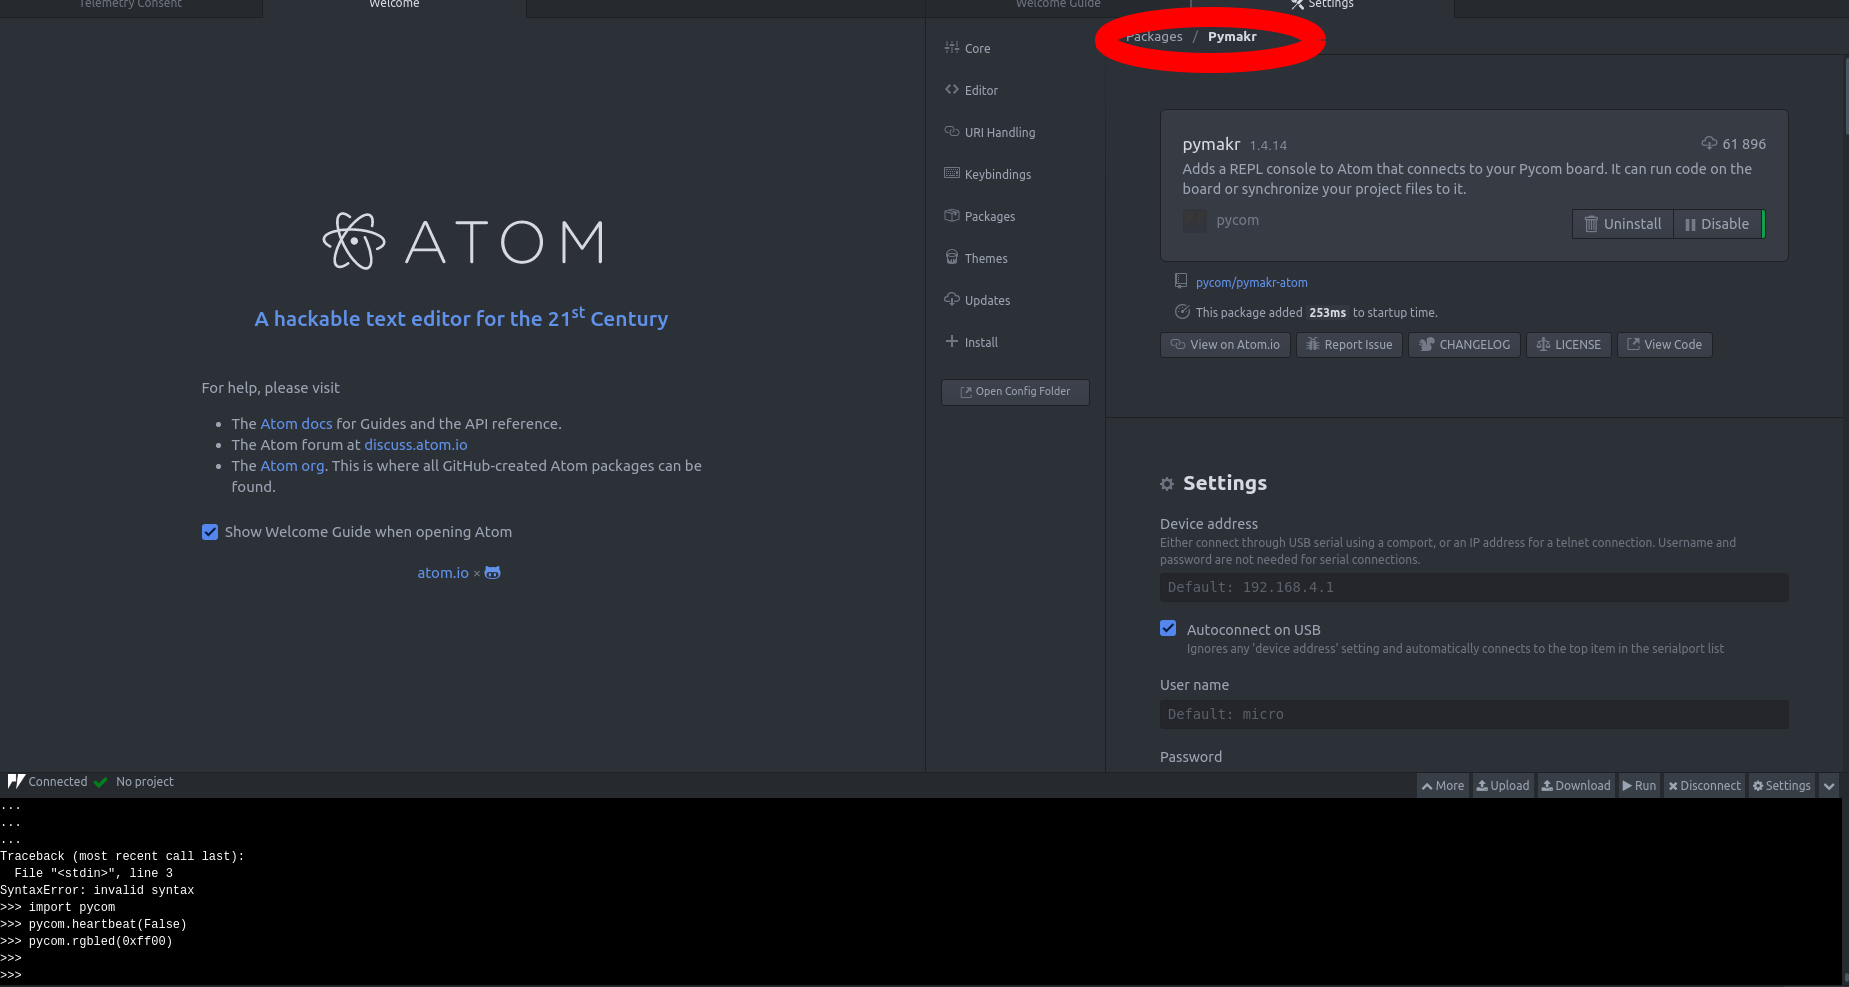
\includegraphics[keepaspectratio=true,scale=0.2]{atom.png}
\label{visina8}
\end{center}\end{figure}

Si il est impossible d'installer pymakr, essayez d'installer une version antérieure à : \url{https://github.com/atom/atom/releases},
Une alternative est aussi Visual Studio Code.


\subsubsection{Connexion à la carte}

Déterminer le port série sur lequel la carte est montée :

Après le branchement : 

\begin{minted}{bash}
dmesg | grep tty 
\end{minted}

ttyACM0 dans mon cas




\subsubsection{Pour ouvrir les ports ttyACM0 et ttyACM1 }

\textbf{Solution temporaire} 


\begin{minted}{bash}
sudo chmod 666 /dev/ttyACM0
\end{minted}
Il faut le entrez cette commande souvent. \\
\textbf{Solution permanente}\\

Créer un fichier dans son home

\begin{minted}{bash}
50-myusb.rules
\end{minted} 

l'éditer : 

\begin{minted}{bash}
KERNEL=="ttyACM[0-9]*",MODE="0666"
\end{minted}

Puis copiez ce fichier dans /etc/udev/rules.d/ et redémarrer votre PC.\\

\begin{minted}{bash}
 sudo cp 50-myusb.rules /etc/udev/rules.d
\end{minted}
C'est suffisant pour ne plus avoir à réouvrir les ports manuellement. Cependant, n'importe quel dispositif usb connecté au PC a maintenant le droit d'écriture sur le PC. \\

Pour plus de sécurité ajouter ces lignes dans ce fichier :

\begin{minted}{bash}
ACTION=="add", KERNEL=="ttyACM[0-9]*", ATTRS{idVendor}=="xxxx", 
ATTRS{idProduct}=="yyyy", MODE="0666"
\end{minted}
 
 Pour déterminer idVendor et idProduct des cartes tapez lsusb avant et après avoir connecter la carte. \\

 Dans mon cas avant et après avoir branché une carte lopy4 :
 
 \begin{figure}[H]
\begin{center}
\advance\leftskip-3cm
\advance\rightskip-3cm
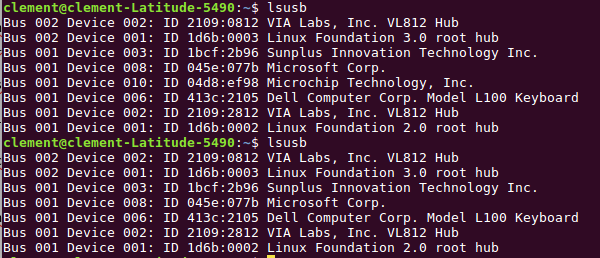
\includegraphics[keepaspectratio=true,scale=0.5]{lsusb.png}
\label{visina8}
\end{center}\end{figure}

idProduct = ef98\\
idVendor= 04d8\\

Pour ajouter d'autres appareils, copier coller ces lignes en changeant idProduct et idVendor. \\


Selon l'image utiliser la console d'Atom pour se connecter à la carte :



  \begin{figure}[H]
\begin{center}
\advance\leftskip-3cm
\advance\rightskip-3cm
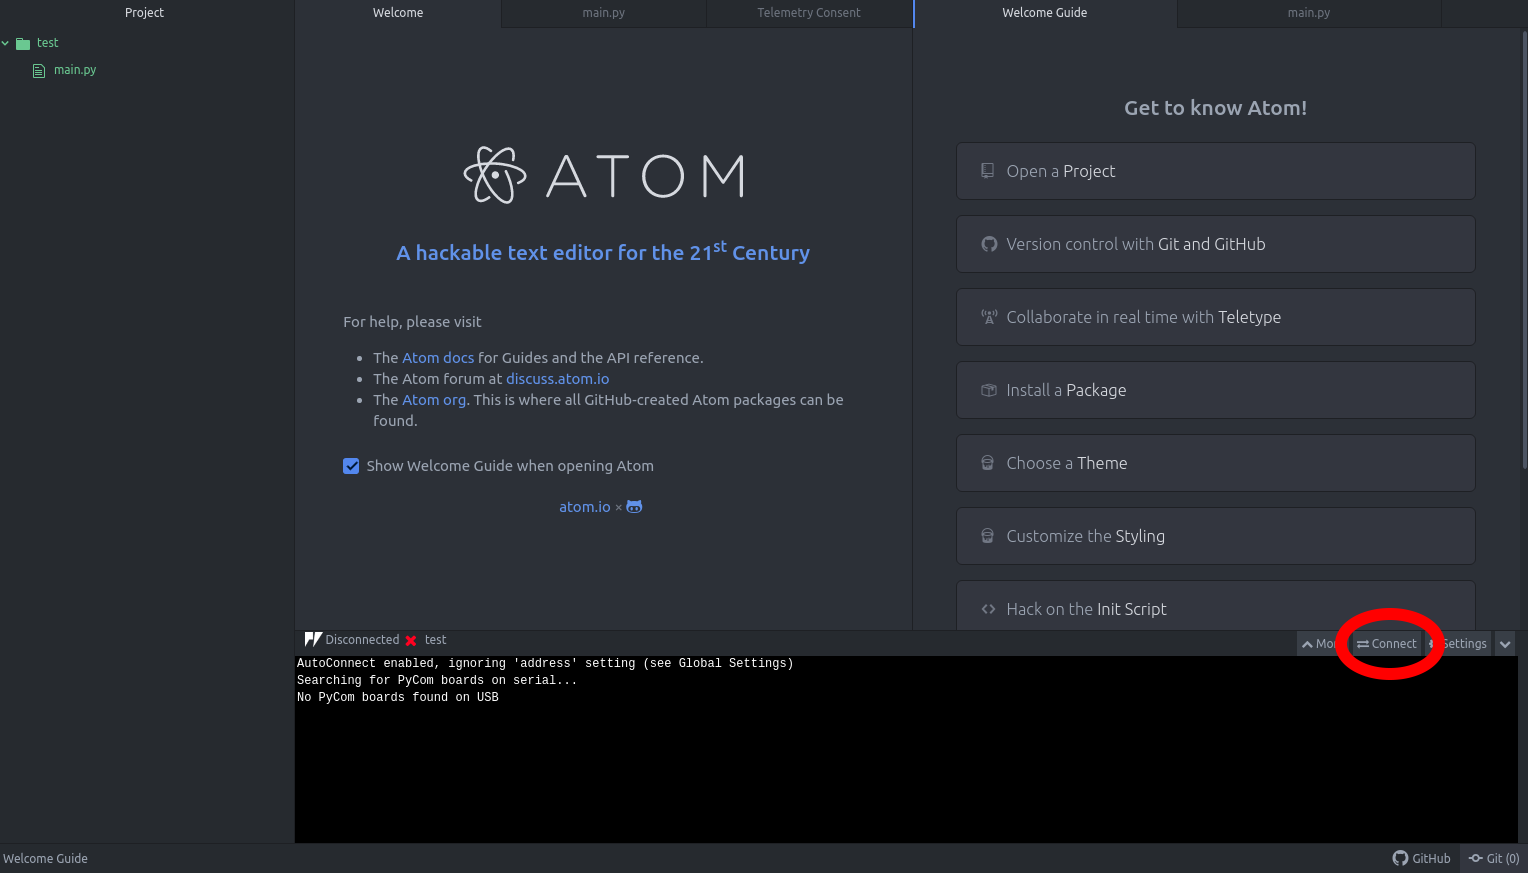
\includegraphics[keepaspectratio=true,scale=0.3]{atom_connect.png}
\label{visina8}
\end{center}\end{figure}


\subsection{Télécharger un firmware sur la carte avec Atom Pymakr}
Téléchargez le code à \url{https://github.com/GitClementtest/lopy4_rgbled} \\
%Guide sur le site d'atom : \url{https://docs.pycom.io/gettingstarted/programming/first-project/}

%Créer un répertoire dans mon cas RGB-LED. Y créer main.py 
Ouvrir ce projet avec ATOM

main.py :
 \begin{minted}{python}
    import pycom
    import time

    pycom.heartbeat(False)

    while True:
        pycom.rgbled(0xFF0000)  # Red
        time.sleep(1)
        pycom.rgbled(0x00FF00)  # Green
        time.sleep(1)
        pycom.rgbled(0x0000FF)  # Blue
        time.sleep(1)
        
    \end{minted}

Dans Atom File, Open Folder pour choisir son projet puis cliquer sur Upload dans la console Pymakr pour télécharger le  code sur la carte. \\



\begin{figure}[H]
\begin{center}
\advance\leftskip-3cm
\advance\rightskip-3cm
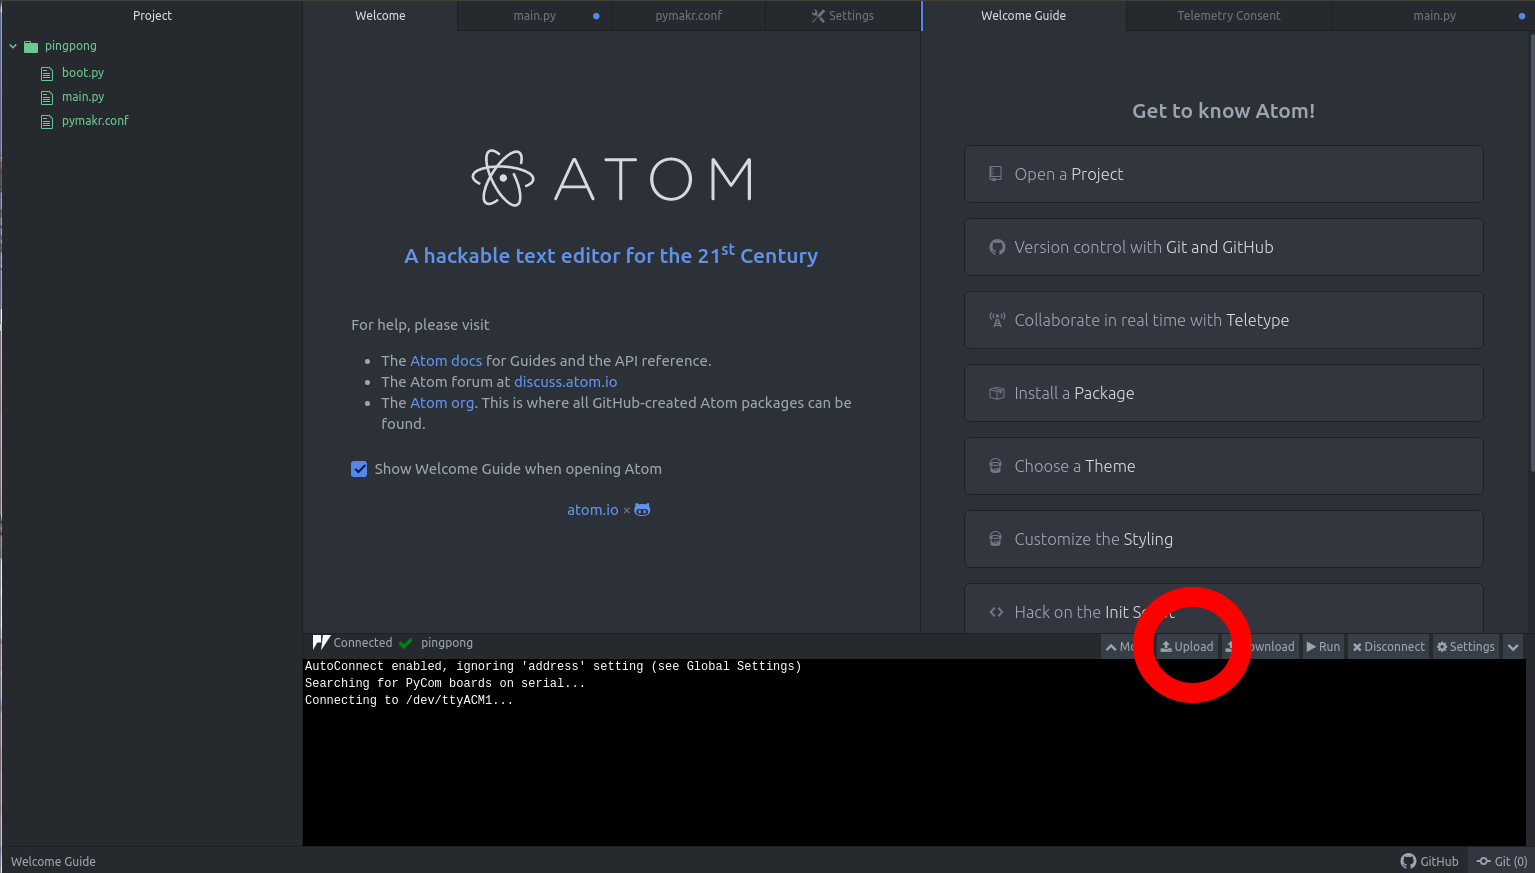
\includegraphics[keepaspectratio=true,scale=0.3]{atom_upload.png}
\label{visina8}
\end{center}\end{figure}

\textbf{Attention aux identations} pour le firmware. Parfois avec des copier-coller les indentations se perdent.
Il faut coller toutes les lignes à gauche du fichier (colonne 0), sauf lorsqu'on entre dans des conditions type while, if etc. Dans ces conditions il faut 1 tabulation au début de chaque ligne.
Si ce n'est pas respecté le programme ne compile pas. \\


Après avoir téléchargé le firmware sur la carte, appuyer sur le bouton reset de la carte à côté des leds rgb pour lancer le programme.

\begin{figure}[H]
\begin{center}
\advance\leftskip-3cm
\advance\rightskip-3cm
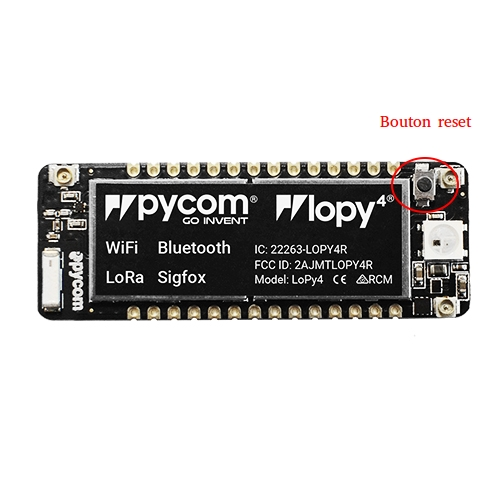
\includegraphics[keepaspectratio=true,scale=0.3]{reset.jpeg}
\label{visina8}
\end{center}\end{figure}

\subsection{Avec un terminal série type PuTTY}

PuTTY : sélectionner liaison série, choisir le bon port /dev/ttyACM0 dans mon cas, baudrate 115200.


\section{Applications LoraWan}


\textcolor{red}{Branchez l'antenne LoRa avant d'alimenter la carte sinon la carte grille}\\

Brancher l'antenne selon l'image :

 \begin{figure}[H]
\begin{center}
\advance\leftskip-3cm
\advance\rightskip-3cm
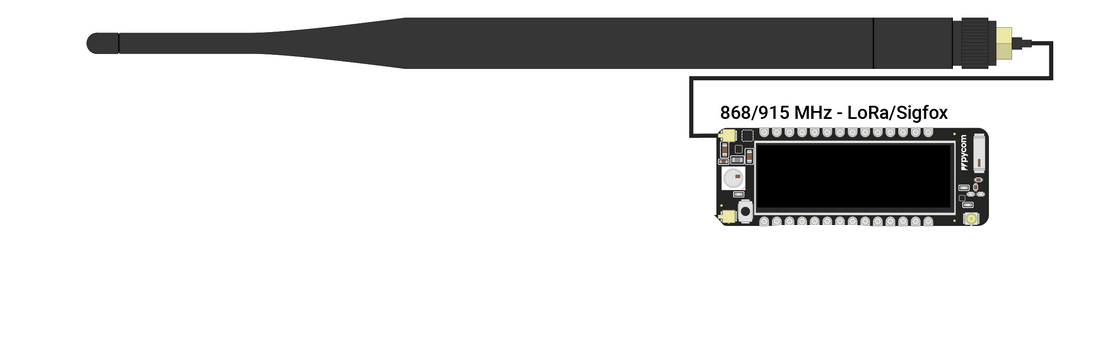
\includegraphics[keepaspectratio=true,scale=0.3]{antennes_lopy.png}
\label{visina8}
\end{center}\end{figure}



Exemple 2 cartes qui communiquent entre elles.
\\

%Seule l'antenne 868 MHz est utile pour l'exemple.

\subsection{Code à télécharger sur les cartes}

Code disponible à ce lien : \url{https://github.com/GitClementtest/lopy4_loramac}\\
%Carte A

%\begin{minted}{python}

%from network import LoRa
%import socket
%import time

%# Please pick the region that matches where you are using the device:
%# Asia = LoRa.AS923
%# Australia = LoRa.AU915
%# Europe = LoRa.EU868
%# United States = LoRa.US915
%lora = LoRa(mode=LoRa.LORA, region=LoRa.EU868)
%s = socket.socket(socket.AF_LORA, socket.SOCK_RAW)
%s.setblocking(False)

%while True:
%    if s.recv(64) == b'Ping':
%        s.send('Pong')
%    time.sleep(5)


%\end{minted}


%Carte B
Télecharger ce code sur 2 cartes Lopy avec antenne LoRa.

%\begin{comment}
\begin{minted}{python}
from network import LoRa
import socket
import machine
import time

# initialise LoRa in LORA mode
# Please pick the region that matches where you are using the device:
# Asia = LoRa.AS923
# Australia = LoRa.AU915
# Europe = LoRa.EU868
# United States = LoRa.US915
# more params can also be given, like frequency, tx power and spreading factor
lora = LoRa(mode=LoRa.LORA, region=LoRa.EU868)

# create a raw LoRa socket
s = socket.socket(socket.AF_LORA, socket.SOCK_RAW)

while True:
    # send some data
    s.setblocking(True)
    s.send('Hello')

    # get any data received...
    s.setblocking(False)
    data = s.recv(64)
    print(data)

    # wait a random amount of time
    time.sleep(machine.rng() & 0x0F)




\end{minted}
%\end{comment}

\section{Résultat}

\subsection{Putty}
Pour l'installer :

\begin{minted}{bash}
sudo apt-get install putty
\end{minted}

Ouvrez des liaison séries avec putty ttyACM0 et ttyACM1, speed 115200.
Ne pas oublier d'ouvrir les ports avec sudo chmod 666 /dev/ttyACM0 si ce n'est pas fait \\
Appuyer sur reset si le programme ne démarre pas.\\

Les cartes vont s'échanger des données selon l'image :

\begin{figure}[H]
\begin{center}
\advance\leftskip-3cm
\advance\rightskip-3cm
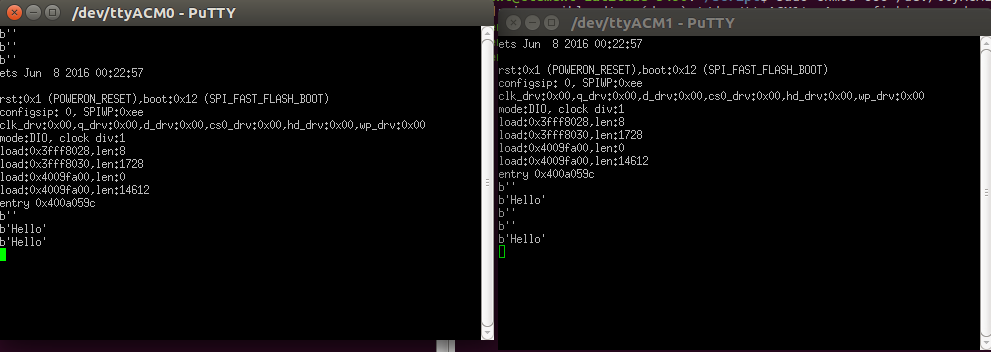
\includegraphics[keepaspectratio=true,scale=0.5]{loramc_lopy.png}
\label{visina8}
\end{center}\end{figure}

\subsection{Avec minicom}
Je recommande d'utiliser minicom car on a pas besoin de réouvrir le programme à chaque fois qu'on déconnecte un appareil.

\subsubsection{Installer minicom}
\begin{minted}{bash}

sudo apt-get install minicom

\end{minted}

\subsubsection{Pour quitter minicom}


\begin{minted}{bash}

ctrl+a puis q
\end{minted}

\subsubsection{lancer minicom}
\begin{minted}{bash}
sudo minicom

\end{minted}


\subsubsection{Configurer minicom}
\begin{minted}{bash}

sudo minicom -s
\end{minted}

\section{Résultat}
\begin{figure}[H]
\begin{center}
\advance\leftskip-3cm
\advance\rightskip-3cm
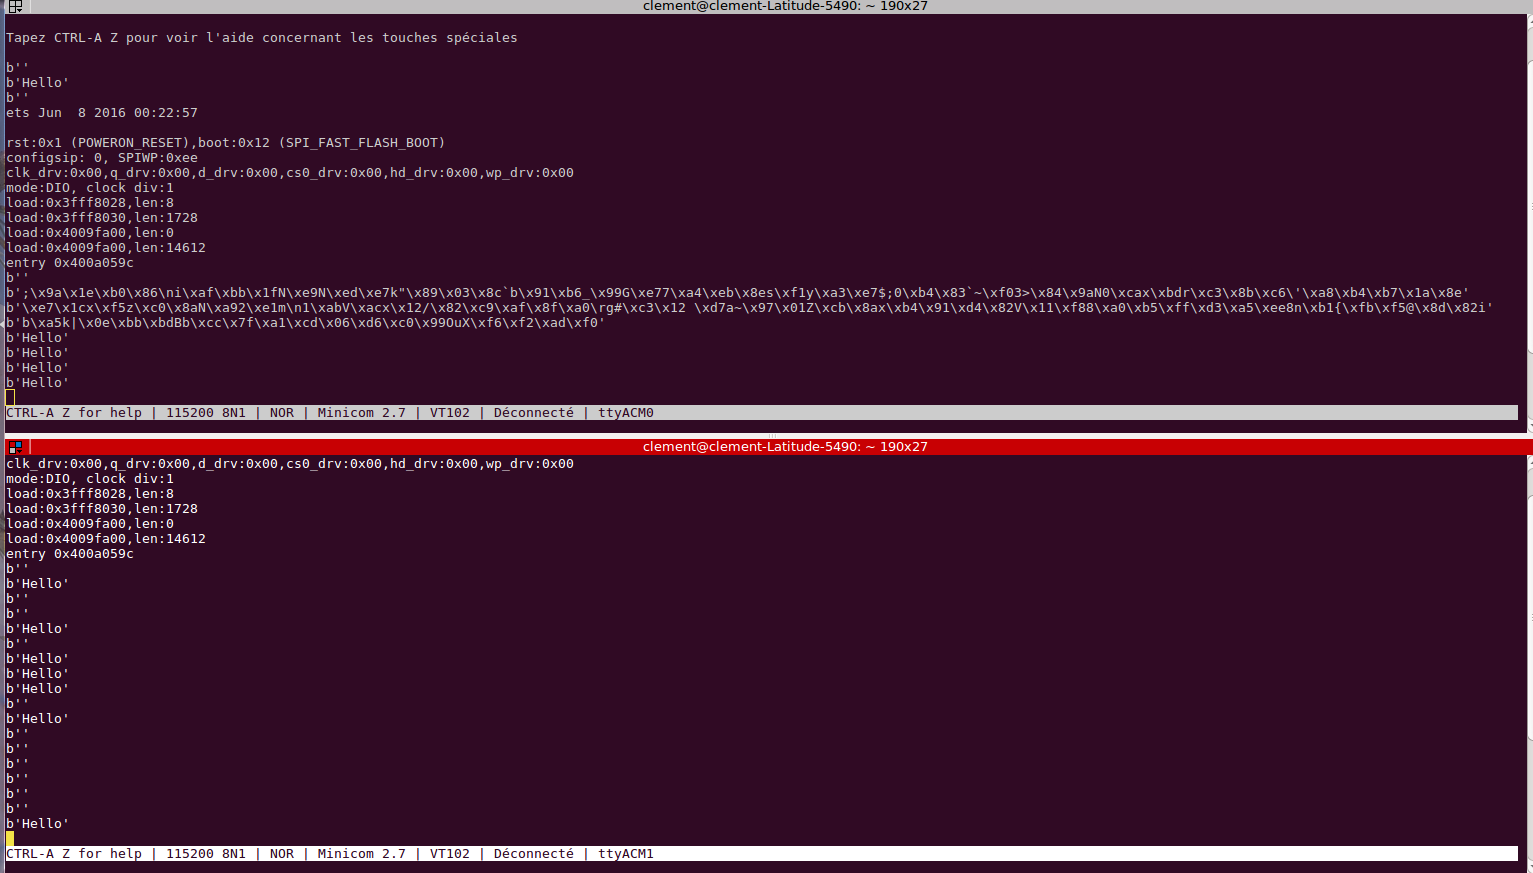
\includegraphics[keepaspectratio=true,scale=0.4]{minicom_loramac.png}
\label{visina8}
\end{center}\end{figure}





\end{document}
